In Figure \ref{fig:T90_comparison} of Section \ref{sec:selecting_common_GRBs}, it was noted that some GRBs have systematically smaller $\T$ in \f\ than \s. Hence, Figure \ref{fig:T90_comparison} was re-plotted as Figure \ref{fig:T90_vs_T90}, with the traditional demarcation lines of `long' and `short' GRBs clearly indicated, to aid the eye. It is observed that for $11$ GRBs, the ratio between the \f\ and \s\ $\T$s is significantly different from unity. A few questions arise naturally: Is there any systematic effect of the way these instruments detect GRBs, for example their wavebands and sensitivities? Does the way the different classes of GRB evolve also play a role in introducing this discrepancy? Or are we actually looking at a different, `intermediate' class of GRBs \citep{Horvath_&_Toth-2016-Ap&SS}? 

\begin{figure}
\begin{center}
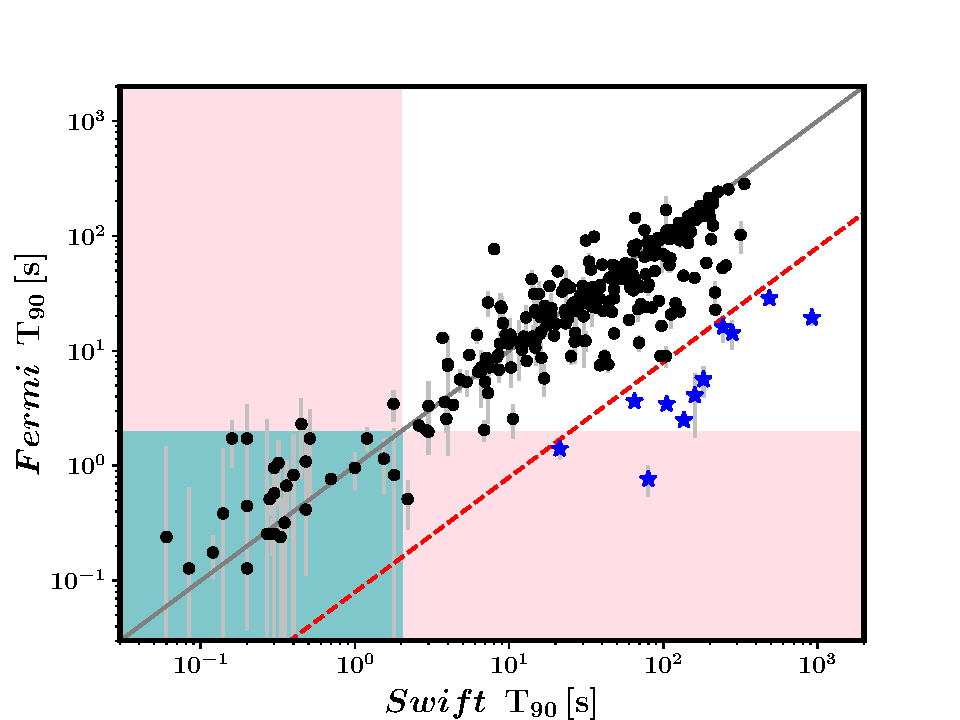
\includegraphics[scale=0.5]{T90_vs_T90--all}
\caption[Detailed comparison of $\T$s of \f\ and \s\ GRBs]{For the $265$ GRBs detected with both \s\ and \f\ in the $\sim 9$ years of operation. The green patch shows those which are ``short'' [$2$ s criterion] in both, the pink patches show those which are long in one but short in the other. The gray line is what would happen in the ideal world: the $\T$s would be equal. It is observed that systematically more number of GRBs have smaller $\T$ for \f\ than \s. In fact, if a cut of $10$ is placed on the ratio motivated by one GRB which is certainly long in \s\ while short in \f, it is seen that $11$ GRBs fall below that line.}
\label{fig:T90_vs_T90}
\end{center}
\end{figure}

First I confirmed that there are GCNs reporting the detection of all of the $11$ GRBs for both \f -GBM and the \s -BAT. Then I looked for reports in the literature which mention any of these GRBs in particular. There is no published paper reporting detailed analysis of $10$ out of $11$ of these GRBs, the exception being GRB 080928 [\s\ nomenclature] / GRB080928628 [\f\ nomenclature].

\cite{Rossi_et_al.-2011-A&A} have done a thorough analysis of the \s\ as well as \f\ data to make a decisive statement about the peculiarity of this GRB: it had already started emitting its ``afterglow'' emission in the optical wavelengths while still giving out ``prompt'' emission in the gamma rays. In fact, it was detected by the $\s$-BAT $204$ s before the \f -GBM trigger, as demonstrated in their Figure 1 and Equation 1. It appears from their Figure 1 that a secondary burst occurred after $204$ s of the first BAT detection, which was the only one detected by \f -GBM. From a quick-look at the \s\ lightcurves\footnote{\url{http://www.swift.ac.uk/burst_analyser/}}, it becomes immediately clear that the BAT and XRT [X-ray Telescope] on-board \s\ detected the rising part of the secondary flare that is also detected by \f, simultaneously. Thus, the greater sensitivity of \s\ ensured that it observed a flare in BAT much before \f\ detected the secondary, independent flare. This secondary flare was also observed by XRT because \s\ had slewn towards the direction of this GRB in the $204$ s between the primary and the secondary flares.

Looking at the common catalogue data shows that except this GRB, the difference in the trigger times for the two detectors is in most cases consistent with $0$, in a few cases going up to maximum of $4$ s. A thorough, manual check in the data for the common catalogue, as well as the original data files used for creating this catalogue validates the time difference for each of these $10$ GRBs. This indeed raises questions worth considering: Are these GRBs systematically softer, so that \f, which calculates the $\T$ in the $50$-$300$ keV waveband instead of $\s$'s $15$-$150$ keV waveband, measures systematically smaller $\T$s? Does the relative sensitivities of the two instruments play a role in this observed artefact? Or is the effect real?

Investigating the quick-look BAT and XRT lightcurves\footnote{\url{http://www.swift.ac.uk/burst_analyser/}} of each of the $10$ GRBs, it is noted that the relative sensitivities of \f\ and \s\ does account for the difference in the measured $\T$s. Since \s\ slews its pointing axis towards the burst direction within a minute or two, the sensitivity of \s -BAT improves with time after the trigger, resulting in it observing not only the prompt emission, but also the afterglow emission that is also detected by XRT. That is, \s\ detects a secondary [late-time] softer X-ray flare which \f\ misses out on because of its poorer sensitivity. Hence, \s\ reports a larger empirically measured $\T$ for these GRBs than \f.

\section*{Conclusions}
%We conclude that a small sub-sample of GRBs common to \s\ and \f\ exist. Except one GRB in which the discrepancy is due to the sensitivity of \s\ and \f, all the other bursts emit secondary soft X-ray flares that are detected only by \s\ but not by \f, explaining the difference in the $\T$s empirically measured by these two instruments.

We have examined the empirically derived durations ($\T$s) of the sample of GRBs common to \s\ and \f. A good fraction of the sample seems to have systematically higher durations inferred by \s -BAT than \f -GBM. This is expected, due to the fact that \s -BAT calculates the duration of GRBs in a lower energy window than \f -GBM, and also because it is more sensitive than \f -GBM at these energies. However, for a small sub-sample, the difference in the $\T$s is significant. It is known that the XRT on-board \s\ detects secondary flares for a fraction of \s -GRBs. Our analysis of the simultaneous lightcurves of \s -BAT and \s -XRT shows that BAT also records these secondary flares for this sub-class of GRBs. This indicates that they form a separate class, and it is worth investigating them further. The analysis of comparing the independent duration estimates of GRBs detected by different missions is thus capable of identifying these interesting GRBs.